\documentclass[a4paper, margin=1in]{article}
%\usepackage{CJK}
\usepackage{latexsym}
\usepackage{color}
\usepackage[x11names]{xcolor} % for a set of predefined color names, like LemonChiffon1
\usepackage{graphicx, float}\usepackage{graphicx}
\usepackage{algorithmic}
\usepackage{algorithm}
%\usepackage{algpseudocode}
%\usepackage[colorlinks]{hyperref}
\usepackage[toc,page]{appendix}
\usepackage{bm}
\setlength{\oddsidemargin}{-0.0in}
\setlength{\evensidemargin}{-0.0in} \setlength{\textwidth}{6.0in}
\setlength{\textheight}{9.0in} \setlength{\topmargin}{-0.2in}
%\usepackage[boxruled]{algorithm2e}

%\setlength{\leftmargin}{0.7in}
\usepackage{amssymb, graphicx, amsmath}  %  fancyheadings,
\usepackage{setspace}
\newcommand\qed{\qquad $\square$}
\newcommand{\nn}{\nonumber}

\usepackage{lipsum}

\usepackage{listings}
\lstset{
  basicstyle=\ttfamily,
  columns=fullflexible,
  frameround=fttt,
  breaklines=true,
  %postbreak=\mbox{\textcolor{red}{$\hookrightarrow$}\space},
}

\definecolor{mGreen}{rgb}{0,0.6,0}
\definecolor{mGray}{rgb}{0.5,0.5,0.5}
\definecolor{mPurple}{rgb}{0.58,0,0.82}
\definecolor{backgroundColour}{rgb}{0.95,0.95,0.92}

\lstdefinestyle{CStyle}{
basicstyle=\ttfamily,
language=C,
numberstyle=\tiny\color{mGray},
numbers=left,
frame=lines,
framexleftmargin=0.5em,
framexrightmargin=0.5em,
backgroundcolor=\color{LemonChiffon1},
showstringspaces=false,
escapeinside={(*@}{@*)},
}

\def \[{\begin{equation}}
\def \]{\end{equation}}
\def\proof{{\bf Proof:\quad}}
\def \endzm {\quad $\Box$}
\def\dist{\hbox{dist}}

\usepackage{tabularx,booktabs}
\newcolumntype{C}{>{\centering\arraybackslash\hsize=.5\hsize}X} % centered version of "X" type
\setlength{\extrarowheight}{1pt}
\usepackage{caption}% <-- added


\newcommand{\R}{\mathbb{R}}
%\newtheorem{yinli}{����}[section]
\newcommand{\D}{\displaystyle}
\newcommand{\T}{\textstyle}
\newcommand{\SC}{\scriptstyle}
\newcommand{\FT}{\footnotesize}

\usepackage{hyperref}
\newcommand\fnurl[2]{%
  \href{#2}{#1}\footnote{\url{#2}}%
}


%\newtheorem{theorem}{Theorem}[section]
%\renewcommand{\thetheorem}{\arabic{section}.\arabic{theorem}}
\newtheorem{definition}{Definition}
\renewcommand{\thedefinition}{\arabic{section}.\arabic{definition}}
\newtheorem{lemma}{Lemma}[section]
\renewcommand{\thelemma}{\arabic{section}.\arabic{lemma}}
\newtheorem{remark}{Remark}
\renewcommand{\theremark}{\arabic{section}.\arabic{remark}}
\newtheorem{proposition}{Proposition}[section]
\renewcommand{\theproposition}{\arabic{section}.\arabic{proposition}}
\newtheorem{corollary}{Corollary }[section]
\renewcommand{\thecorollary}{\arabic{section}.\arabic{corollary}}
\renewcommand{\theequation}{\arabic{section}.\arabic{equation}}
\renewcommand{\baselinestretch}{1.35}
\newtheorem{exam}{Example}[section]
\renewcommand{\theexam}{\arabic{section}.\arabic{exam}}
\newtheorem{theo}{Theorem}[section]
\renewcommand{\thetheo}{\arabic{section}.\arabic{theo}}

\usepackage{enumitem}
\newenvironment{QandA}{\begin{enumerate}[label=\bfseries\alph*.]\bfseries}
	{\end{enumerate}}
\newenvironment{answered}{\par\normalfont}{}

% Define a \HEADER{Title} ... \ENDHEADER block
\makeatletter
\newcommand{\HEADER}[1]{\ALC@it\underline{\textsc{#1}}\begin{ALC@g}}
\newcommand{\ENDHEADER}{\end{ALC@g}}
\makeatother

\newcommand{\argmin}{\operatornamewithlimits{argmin}}
\newcommand{\argmax}{\operatornamewithlimits{argmax}}

\usepackage{url} % to make url in bibtex shows up

% Create a command to cleanly insert a snippet with the style above anywhere in the document
\newcommand{\insertcode}[2]{\begin{itemize}\item[]\lstinputlisting[caption=#2,label=#1,style=CStyle]{#1}\end{itemize}} % The first argument is the script location/filename and the second is a caption for the listing

\begin{document}
%\begin{CJK*}{GBK}{song}

\begin{center}

{\LARGE \bf CS380L: Advanced Operating Systems Lab \#3}\\

\vskip 25pt
 {Zeyuan Hu \footnote{30 hours spent on this lab.}, iamzeyuanhu@utexas.edu }\\
\vskip 5pt
{\small EID:zh4378 Spring 2019 }

\end{center}

\begin{spacing}{1.5}
\section{Environment} \label{environment}

Unless otherwise noted, we use a Linux server for all the experiments. The server has 4 Intel(R) Xeon(R) CPU E3-1220 v5 @ 3.00GHz processors and 16GB of memory, and runs Ubuntu 16.04.2 LTS (kernel version 4.11.0).

\section{ELF Format}

Executable and Linkable Format (ELF) is a file format for executable, object code, shared libraries, and core dump on UNIX-like systems  \cite{elf_wiki}. ELF format taken from \cite{elf_doc} is shown in Figure \ref{elf_format}. An ELF binary 
starts with a fixed-length \textit{ELF header}, which holds a ``road map" describing the file's organization (e.g., instruction set architecture, endianness, system ABI, entry point of the program). A \textit{program header table}, if present, tells the system how to create a process image (i.e., execute a program). Each entry of program header table corresponds to a segment in the virtual address space. Part of the segment contents can be loaded from the executable file, which is also defined in the program header table. A \textit{section header table} contains information describing the file's sections (e.g., \texttt{.text}, \texttt{.data}, \texttt{.rodata}, \texttt{.bss}). Some of them will be loaded into virtual address space as part of segments indicated by program header table. Each entry gives information such as section name, the section size, etc. Program header table is required for to-be-run file and optional for relocatable file; section header table is required for file used during linking and optional for others.

There are some special sections we care about in ELF. \texttt{.text} section contains the program's executable instructions; \texttt{.rodata} represents read-only data, such as ASCII string constants produced by the C compiler; \texttt{.data} holds the program's initialized data, such as global variables declared with initializers like \lstinline|int x = 5;|; \texttt{.bss} section holds uninitialized data (e.g., uninitialized global variables such as \texttt{int x};) that contribute to the program?s memory image. \texttt{.bss} immediately follows \texttt{.data} in memory. C requires that ``uninitialized" global variables start with a value of zero. Thus, the system initializes the data with zeros when the program begins to run. The section occupies no file space (linker records just the address and size of the \texttt{.bss} section). The loader or the program itself must arrange to zero the \texttt{.bss} section.

\begin{figure}
	\centering
	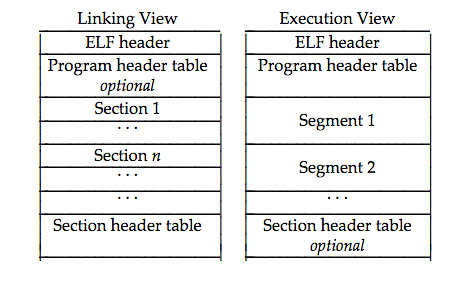
\includegraphics[scale=0.6]{elf_format.png} 
	\caption{ELF format. There are two views of ELF binary: linking view and execution view. Linking view is used during the dynamic linking, whereas execution view is needed when load the program into memory for the program to run.}
	\label{elf_format}
\end{figure}

\section{\texttt{execve} Implementation}

To write our own loader program, we first need to understand how \texttt{execve} system call is implemented in Linux kernel \footnote{we study the source code of Linux 4.8.12}. Essentially, \texttt{execve} performs the heavylifting work of loading a program into memory and start the execution of program as a process in Linux. The main logic of \texttt{execve} is implemented in \lstinline|do_execveat_common| in \texttt{fs/exec.c}. Inside \lstinline|do_execveat_common|, we see the critical function call stack looks like below:

\begin{lstlisting}[style=CStyle]
do_execveat_common
|- exec_binprm
   |- search_binary_handler
      |- load_binary
\end{lstlisting}

For binary with ELF format, \lstinline|load_elf_binary| is registered with \lstinline|load_binary| in \texttt{fs/binfmt\_elf.c}. Thus, we locate the core function \lstinline|load_elf_binary|, which is responsible to load binary with ELF format in the Linux kernel. Further study of the function reveals that the following critical steps are performed in order to load the program into memory and start execution:

\begin{itemize}
	\item Read the ELF header and perform some simple consistency checks. For example, the function checks whether the binary file is executable file (\lstinline|ET_EXEC|) or shared object file (\lstinline|ET_DYN|).
	\item Read the program header table by calling \lstinline|load_elf_phdrs|.
	\item Walk through the entries of the program header table and perform specific actions based on program header table entry type (e.g., \texttt{p\_type}). Note that \lstinline|e_phnum| holds the number of entries in the program header table. Each entry of the table corresponds to a memory segment in the binary file. Kernel is only interested in three types of program header entries during the walk through of the program header table:
	\begin{itemize}
		\item \lstinline|PT_INTERP| entry, which identifies the run-time linker needed to assemble the complete program \cite{oracle_linker}.
		\item \lstinline|PT_GNU_STACK| entry, which determines whether the program's stack should be executable \cite{lwn}.
		\item \lstinline|PT_LOPROC ... PT_HIPROC|, which are values reserved for processor-specific semantics \cite{oracle_linker}.
	\end{itemize}
	\item Once all the program header table entries have been processed, the function performs some checks based on \lstinline|p_type| value it obtained from the previous step (e.g., check for interpreter, check for specific processor architecture).
	\item The function now is ready to set up the new program. The very first step is to call \lstinline|flush_old_exec|, which clears up state in the kernel that refers to the previous program. Some minor setups (e.g., set up program's personality \cite{personality_man}) are performed immediately after. 
	\item \lstinline|setup_new_exec| is called to set up the kernel's internal state for the new program and new credentials for this executable is installed via calling \lstinline|install_exec_creds|.
	\item \lstinline|setup_arg_pages| is invoked to set up kernel's memory tracking structures (e.g., stack \lstinline|vm_area_struct|). This step is part of the goal to set up virtual memory for the new program.
	\item The function now traverse the program header table again and look for entries with type \lstinline|PT_LOAD|, which indicates loadable segments (i.e., areas of the new program's running memory). The entries contain code and data sections that come from the executable file and the size of a \texttt{BSS} section. For each \lstinline|PT_LOAD| entry, the function maps it into the process' address space via \lstinline|elf_map| call and sets up the new program's memory layout accordingly.
	\item \lstinline|set_brk| is invoked to set up zero-filled pages that correspond to the program's BSS \cite{bss} segment.
	\item \lstinline|create_elf_tables| is called to set up the rest of the new program's stack. Basically, the function puts \texttt{argc}, \texttt{argv}, \texttt{envp}, and auxiliary vectors. LWN article \cite{lwn} provides an illustration of the content of the stack set up by the kernel. In addition, Figure 3.11 of System V ABI for \lstinline|x86_64| manual \cite{abi} provides what initial process stack looks like.
	\item \lstinline|start_thread| is invoked to start the execution of the new program.
\end{itemize}
 
\section{User-space Loader}

We leverage \texttt{libfuse} and \texttt{libssh} to implement a network file system. Filesystem in Userspace (FUSE) is a user-space file system framework.  FUSE consists of a Linux kernel module and a user-level daemon. When a user application performs operations on a mounted FUSE file system, the operation will be routed to FUSE's kernel driver by VFS. The operations as requests will be maintained by a queue and user-level daemon will pick a request from the kernel queue and process the request. Daemon will write response back to kernel once it is done with processing.  More information about FUSE can be seen in \cite{vangoor2017fuse}.

\subsubsection{System Architecture}

We implement a network file system. Like NFS, it supports a server with multiple clients. On the client side, the FUSE client program will mount a user-space file system with remote user, remote host, remote path, local cache path, and local mount point provided by the user. Remote user and remote host specify the server that our network file system want to contact. Remote path specifies the location on the server we want to store and fetch files for the clients. Our system requires user to specify a path for local cache as we serve clients' requests from local cache as much as we can. In other words, some file operations are directly served by the local cache without further contact with server. Communications between clients and the server are done via SSH protocol. Thus, there is no server-side implementation in our system. 

\subsubsection{FUSE Calls Implemented}

We implement the following operations: \texttt{getattr}, \texttt{readdir}, \texttt{create}, \texttt{open}, \texttt{read}, \texttt{write}, \texttt{fsync}, \texttt{release}, \texttt{mkdir}, \texttt{unlink}, and \texttt{rmdir} in our system. 
Our operation implementation is based on \texttt{libfuse} version is 2.9.4 \footnote{check via \lstinline|fusermount -V|} API. In \texttt{libfuse}, there are two sets of APIs: a "high-level", synchronous API, and a "low-level" asynchronous API. 
The key difference between "high-level" and "low-level" API is that "high-level" allows us to work with file names and path instead of inodes in synchronous fashion.
Thus, for the simplicity, our implementation adopts the "high-level" API.

\texttt{getattr} operation is used to get attributes of a file or a directory. Function signature of \texttt{libfuse}'s \texttt{getattr} operation is \lstinline|int getattr(const char * path, struct stat * stbuf);|. Our implementation should fill \texttt{stbuf} to contain attributes of file or directory indicated by \texttt{path}. Since \texttt{struct stat} is the same structure used in \texttt{stat} call \cite{stat_man}, we can leverage \texttt{stat} command \cite{stat1_man}.  Specifically, in our implementation, we execute \texttt{stat} command remotely via SSH to collect attributes of the desired target (specified by \texttt{path}). The output of the \texttt{stat} command is parsed on the client side of the file system.  We fill \texttt{st\_size}, \texttt{st\_blocks}, \texttt{st\_mode}, and \texttt{st\_nlink} fields of \texttt{struct stat} from the parse result. \texttt{st\_uid} and \texttt{st\_gid} are filled with UID and GID of the file system client process. \lstinline|st_mode| is filled with \lstinline|644| (i.e., \lstinline|rw-r--r--|) if the target is file and  \lstinline|755| (i.e., \lstinline|rwxr-xr-x|) if the target is directory.

\texttt{readdir} operation is used to get entries in a directory (i.e., read directory). There are two modes
of operation for the implementation: whether we keep track of offset provided as one of function signature argument. If we ignore the offset, the content of whole directory will be read in a single operation. For the simplicity, we ignore the offset in our implementation. This can be troublesome if the content of directory is greater than the supplied buffer size. The key to our implementation is the implementation of filler (with type \lstinline{fuse_fill_dir_t}), which is used to add directory entry to the supplied buffer. In our case, \texttt{getattr} is invoked whenever filler is called. 

\texttt{create} and \texttt{open} operations correspond to \texttt{creat} and \texttt{open} system calls. libfuse's \texttt{open} operation has signature \lstinline|int open(const char* path, struct fuse_file_info* fi);|. \texttt{path} specifies the file to be opened and \texttt{fi->flags} indicates the open flags (same as \texttt{flags} in \texttt{open} system call \cite{open_man}). \texttt{fi->fh} represents file handle, which may be filled for future usage.  In our implementation, when \texttt{open} is invoked, the target file will be downloaded from server via SCP and saved in the local cache path. Operations like \texttt{read}, \texttt{write}, and \texttt{fsync} will be served from local cache copy. The local cache copy is opened with the same flags and corresponding \texttt{fd} is saved in \texttt{fi->fh} for future use. \texttt{create} operation is similar to \texttt{open} except it will first create the file remotely if the file does not exist.

\texttt{read}, \texttt{write}, and \texttt{fsync} operations are served by local cache file copy via \texttt{fi->fh}. Same as NFSv2, we implement flush-on-close semantic for update visibility. Specifically, we do not upload the file to the server on \texttt{write} and \texttt{fsync}, instead we update server's copy when the file is closed. Doing so removes network communication overhead between each file update, but we may face file inconsistency if there are multiple clients updating the same file competitively. 

\texttt{release} operation is invoked by \texttt{libfuse} when closing a file descriptor. This is the place where we implement flush-on-close semantic. We first close \texttt{fi->fh}, which is the file descriptor the local cache copy. Then, we upload the local cache copy to the server via SCP.

\texttt{mkdir}, \texttt{rmdir}, and \texttt{unlink} operations are performed by executing \texttt{mkdir} and \texttt{rm} command remotely via SSH.

\subsubsection{Limitation}

Our implementation has coarse-grained access control in the sense that all the files and directories have the same UID, GID, and permission mask. To enable a more fine-grained access control, we could use a file similar to \texttt{/etc/exports} in NFS to indicate what ip address can have what access (read, write, or both) to what directories and files. Doing so requires us to implement a server-side code as a guard to perform identity check. However, access control is orthogonal to our experiment goal and we left this feature as future work.

Incomplete file metadata also impacts how we implement the file consistency mechanism. In our implementation, we do not keep creation time, access time, and modification time of directories and files. As a result, we cannot selectively perform SCP on \texttt{open}: if we maintain file stats, we can perform stats comparison between remote copy and cached copy to see whether we need to perform expensive data transmission over the network. In addition, since we only SCP file during \texttt{open}, file can change between \texttt{open} and \texttt{read}. NFS periodically issues \texttt{getattr} to server to ensure cache consistency. Since we do not support file timestamp, we cannot issue \texttt{getattr} periodically and let \texttt{read} directly read from server when the local cache is invalidated.  

Some other issue might exist regarding file consistency. For example, we implement the last-writer-wins policy: if a file is updated by the multiple users, the last one who close the file will keep its change to the file on server. However, this might be troublesome. A more sophisticated method is to automatically merge change to the file whenever possible and maintain multiple versions of files on the server with each version associated with its owner. Other versions may not be visible the user and only a specific system command issued will make those versions visible. We also allows a file can be opened multiple times. This is troublesome as later open operations can overwrite changes made by previous file descriptors. One possible fix is to only download copy file from server when there is no local cache copy or implement a copy-on-write mechanism: each open will lead to a unique version of the file and it is up to user to resolve potential conflicts. 

\subsection{Evaluation}

In this section, we compare our network file system with NFS under three workloads.

\subsubsection{Experiment Setup}

For our network file system, we use \lstinline|thoothukudi-lom| as client and \lstinline|erode-lom| as server. On the client side, our system is mounted under \lstinline|/tmp/barfs| and the local cache is under \lstinline|/tmp/barfs_cache|. For NFS, to make a fair comparison, we also use memory as storage location for NFS server and we require the NFS to reply requests only after changes have been committed to stable storage (\lstinline|sync|) \cite{exports_man}. Our \lstinline|/etc/exports| looks like below:

\begin{lstlisting}[style=CStyle]
/tmp/nfs *(rw,sync,no_subtree_check,no_root_squash)
\end{lstlisting}

On the client side, we mount our NFS client under \lstinline|/tmp/nfs| as following:

\begin{lstlisting}[style=CStyle]
sudo mount -t nfs -o sync 192.168.1.120:/tmp/nfs /tmp/nfs
\end{lstlisting}

As pointed out earlier, \lstinline|192.168.1.120| refers to \lstinline|thoothukudi-lom|.

\subsubsection{Workloads and Results}

We use three workloads to compare our network file system with NFS. We measure the total amount of time spent on file creation (\texttt{creation}), file open (\texttt{open}), file write (\texttt{write}), and file close (\texttt{close}). The detailed description of workloads and corresponding results follow:

\textbf{1. Random writes.} We create a 100MB file with random bytes in it. Then, we perform $10^5$ 4KB random writes to the created file. Note that by random writes, we mean the offset of the file is chosen randomly when write. The performance of our network file system and NFS is shown in Figure


As shown in the figure, we observe our networked file system spent more time when open the file (3 seconds vs. almost instant in NFS). This is expected as we download file from remote each time we open a file. In contrast, NFS seems to only create local copy on open when there is no modification to the file yet. There is a dramatic performance difference when come to write. Compared to our network file system, NFS spent around 440 seconds to finish writes. This difference is reasonable as we require NFS to synchronously update the local change with the remote server whereas ours only performs write into local copy. Our network file system also performs well on close due to the synchronization work need to be done by NFS.

\textbf{2. Sequential writes.} In this workload, we first create an empty file. Then we we repeatedly append 4KB data to file (i.e., sequential writes) until the file size reaches 500MB. The performance of two systems is shown in Figure \ref{sequential_writes}.

\begin{figure}
	\centering
	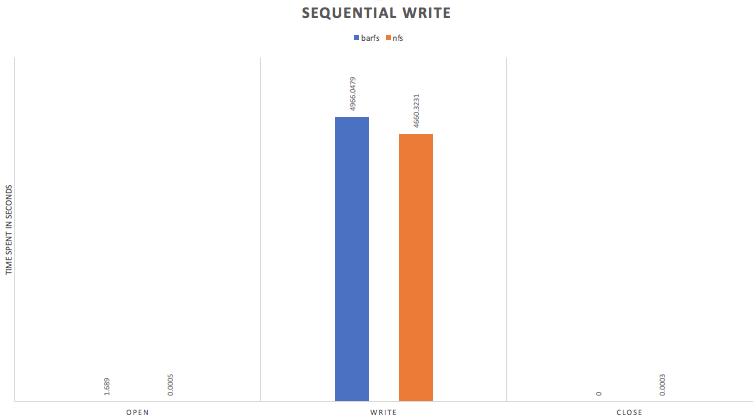
\includegraphics[scale=0.6]{sequential_writes.png} 
	\caption{Performance of NFS and our network file system under sequential writes workload}
	\label{sequential_writes}
\end{figure}

Since we create an empty file, there is no noticeable difference between NFS and our network file system on \texttt{open}. In addition, since the major performance bottleneck \texttt{release} is called after \texttt{close}, our network file system \texttt{close} is done almost immediately. For NFS close case, since the write is already synchronized to the server, there is no much work need to be done. The major difference between two systems under this workload is the \texttt{write} part. NFS takes less time finish writing than our networked file system (4660 seconds vs. 4966 seconds). The major overhead from our network file system is the FUSE framework which cross kernel boundary multiple times whereas NFS sits in the kernel space. However, the gap is offset by our design: \texttt{fsync} after each write forces NFS to synchronize with the remote server. However, in our system, we only synchronize to the remote on \texttt{close}. This is a tradeoff we play when we design our system: we trade file availability with the performance. Unlike NFS, when \texttt{fsync} is called, our system only synchronizes writes to local disk storage. In other words, without closing file, there is only one copy sitting on the client side. If client is crashed and un-recoverable, the file is gone. However, for NFS, the file is still safe as it already synchronizes with the server. Another motivation for our design of \texttt{fsync} is to reduce conflict in the concurrent writes. we think all the writes before \texttt{close} are "unofficial" and should not become visible to other users by uploading it to the server.

\textbf{3. File creation.} In this workload, we create 100 4KB files. The performance of two systems is shown in Figure \ref{file_creation}. 
As shown by the figure, our system takes much more timer creating file than NFS does (49 seconds vs. almost 0 seconds). This meets our expectation because of overhead imposed by the remote file downloading. However, NFS will only create files in local cache and synchronize changes at the background.
When file is closed, NFS will initiate the synchronization to the remote.

\begin{figure}
	\centering
	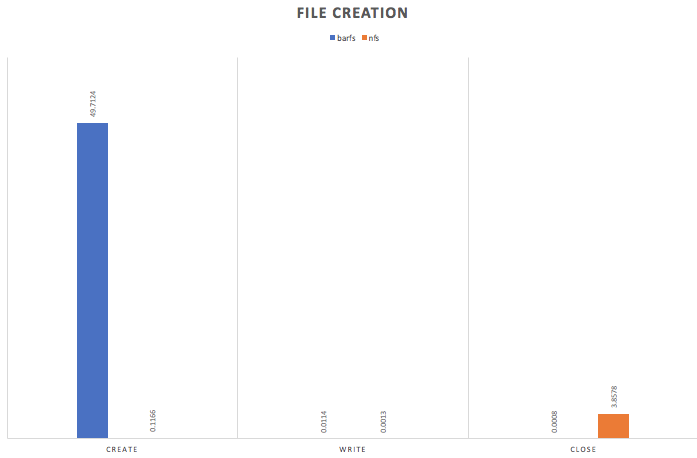
\includegraphics[scale=0.6]{file_creation.png} 
	\caption{Performance of NFS and our network file system under file creation workload}
	\label{file_creation}
\end{figure}

As we can see from workloads, our network file system has performance advantage over NFS when write to the file at the sacrifice of potential file loss.
However, our network file system performs poorly when \texttt{open} operation is involved as remotely downloading file from server is inevitable.

\subsubsection{vs. NFS}

From the design and actual experiment, our network file system shares great similarities with NFS: both of them are stateless and are designed under the assumption of not many concurrent accesses in a one-server-multiple-clients setting. Both of systems implement last-writer-wins policy.

NFS has advantage in terms of file consistency and expensive remote file downloading is avoided with the help of attibute cache and file cache. Attributes cache periodically checks with remote and ensure the file cache is valid at the best effort (client can still with stale copy if the file is changed during the interval between attribute check). In addition, NFS consistently synchronize local writes to the remote to avoid serious consequence of local client power loss. On the other hand, since we follow the principle of frugality (use the least powerful solution to a given problem) \cite{massalin1989threads}, our network file system can reap some performance gain during read and write. Specifically, we only synchronize local copy with remote on close and work with local cache most of time, we avoid overhead during the basic I/O operations.

\section{System Tools Exercise}

\subsection{strace}

\texttt{script} command allows user to record terminal printout into a file \cite{script_man}. Per the lab instruction, we use \texttt{strace} to trace the syscalls and signals of a target process \cite{strace_man}. In our case, we trace the process involving \texttt{cat}. One thing I notice is that \texttt{script} contains some unicode as shown in Figure \ref{session_processed}. Thus, we use the following code to clean up the output:

\begin{lstlisting}[style=CStyle]
cat $FILE | perl -pe 's/\e([^\[\]]|\[.*?[a-zA-Z]|\].*?\a)//g' | col -b > $FILE-processed
\end{lstlisting}

The result is shown in Figure \ref{session_processed} \footnote{raw output and cleanup output comes with the report as \texttt{session\_record} and 
\texttt{session\_record-processed} respectively}. 

\begin{figure}
	\centering
	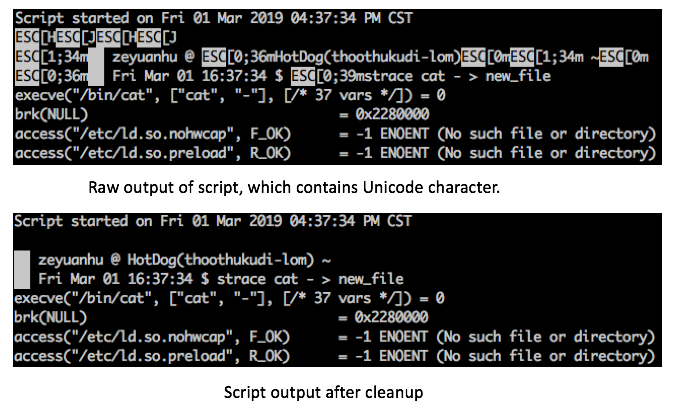
\includegraphics[scale=0.5]{session_record.png} 
	\caption{\texttt{script} output before and after cleanup}
	\label{session_processed}
\end{figure}

\subsection{lsof}

\texttt{lsof} lists all open files \cite{lsof_man}. \texttt{lsof | grep /dev} shows all the open devices used by user-space programs. On our machine, we have the following opened devices:

\begin{itemize}
	\item \texttt{/dev/null}: null device
	\item \texttt{/dev/pts/*} and \texttt{/dev/tty}: terminal devices
	\item \texttt{/dev/urandom}:  kernel random number source device
	\item \texttt{/dev/ptmx}: a character file to create a pseudoterminal master
\end{itemize}

\section{Network Tools}

\texttt{ifconfig} command lists all the network interfaces the machine is using to communicate externally. On our machine, interface for Ethernet is \texttt{eno1}. We can find IP address, gateway address, and subnet mask from the output.

\texttt{tcpdump} command can dump traffic on a network interface.  We use the \texttt{tcpdump} output provided by the lab instruction to answer the questions below.

\begin{QandA}
	\item Are DHCP messages sent over UDP or TCP?
	\begin{answered}
	We use \lstinline!tcpdump -nn -r tcpdump.out.1 | grep -i dhcp! to filter out the DHCP messages from the dump. \lstinline|-nn| ensures that we can see the actual port number instead of the port name. One line of the output is: 
	\begin{lstlisting}
10:19:24.525962 IP 0.0.0.0.68 > 255.255.255.255.67: BOOTP/DHCP, Request from a8:20:66:3b:66:51, length 300
	\end{lstlisting}
	The first field shows the time that the packet was traveling. The second field shows the source host address and port, followed by the destination host address and port. The third field shows the protocl the packet was using. From DHCP \cite{dhcp}, we know DHCP messages sent over UDP. As shown by the printout, the messages are sent between port 68 (client) and port 67 (server).
	\end{answered}
	
	\item What is the link-layer (e.g., Ethernet) address of your host? (Feel free to obscure the last couple bytes for privacy's sake)
	\begin{answered}
	We use the same \texttt{tcpdump} command as above with extra \texttt{-e} option to show linke-layer header. The following printout contains DHCP messages for acquiring IP address:
	\begin{lstlisting}
10:19:24.525962 a8:20:66:3b:66:51 > ff:ff:ff:ff:ff:ff, ethertype IPv4 (0x0800), length 342: 0.0.0.0.68 > 255.255.255.255.67: BOOTP/DHCP, Request from a8:20:66:3b:66:51, length 300
10:19:24.566258 00:21:9b:fb:61:0c > a8:20:66:3b:66:51, ethertype IPv4 (0x0800), length 342: 128.83.158.2.67 > 128.83.158.160.68: BOOTP/DHCP, Reply, length 30
	\end{lstlisting}
	From the printout we can see that the link-layer address (MAC address) of the host is \texttt{a8:20:66:3b:66:51}.
	\end{answered}

	\item What is the IP address of your DHCP server?
	\begin{answered}
		From the printout above, we can see the IP address of DHCP server is 
		\lstinline|128.83.158.2| and the new IP address acquired from DHCP server is \lstinline|128.83.158.160|.
	\end{answered}

	\item What is the purpose of the DHCP release message? 
	\begin{answered}
		DHCP release message is used to release IP address.
	\end{answered}

	\item Does the DHCP server issue an acknowledgment of receipt of the client's DHCP request?
	\begin{answered}
		DHCP server does not issue an acknowledgment of receipt of the client?s release message.
	\end{answered}

	\item What would happen if the client's DHCP release message is lost?
	\begin{answered}
		 If DHCP release message is lost, the DHCP server has to wait for the lease to timeout before assigning it to other clients.
	\end{answered}
\end{QandA}


\end{spacing}
\bibliographystyle{ieeetr}
\bibliography{report}
\end{document}

